\documentclass[12pt,letterpaper]{article}

\usepackage{amsmath, amsthm, amssymb, amsfonts}
\usepackage{graphicx}
\usepackage{bm}
\usepackage{natbib}

\theoremstyle{definition}
\newtheorem{dfn}{Definition}

\begin{document}

% The numbers below controls the amount of space between the following sections
\def\shiftdowna{0.32in}  % Adjust for balance
\def\shiftdownb{0.22in}  % Adjust for balance

% Set up the boiler plate at the top of the page

\begin{center}
\textbf{{\large Project Work Statement}}\\


% SPONSOR
\vspace \shiftdowna
\underline {Sponsor}\\ 
\vspace{5pt}
\textbf{{\large National Marine Fisheries Service}}\\


% TITLE
\vspace \shiftdowna
\textbf{{\large Dungeness Crab Growth}}


% STUDENTS
\vspace{0.35in}
\vspace \shiftdownb
\underline {Participants} \\
\vspace{5pt}
\text{Xiaohan Yang}, \texttt{xyang39@jhu.edu}

% SPONSORS
\vspace \shiftdownb
\underline {Potential Participants}\\
\vspace{5pt}
Bruce Buckson, \texttt{pr.webmaster@noaa.gov} \\
\vspace{3pt}
\text{Tracy Dunn}, \texttt{habitat.conservation@noaa.gov} \\
%\vspace{3pt}
%\text{Glen Coppersmith}, \texttt{coppersmith@jhu.edu}

% DATE
\vspace \shiftdowna
Date: \today

\end{center}

\vfill  
%Fill page to force following note to bottom
\footnoterule
\noindent \small{Any apparent association of this work to National Marine Fisheries Service is
fictional one, and the sole purpose of this work is a class exercise}

\newpage

\section{Background} 
National Oceanic and Atmospheric Administration's National Marine Fisheries Service is a federal agency and a division of the Department of Commerce. It is responsible for the management, conservation and protection of living marine resources and their habitats within the United States' Exclusive Economic Zone (water three to 200 mile offshore). It assesses and predicts the status of fish stocks, makes sure that people obey fisheries regulations, and works to reduce wasteful fishing practices. Under the law of fishing and living things protection, it recovers protected marine species without unnecessarily preventing economic and recreational opportunities. It has six regional offices and eight councils, which help the National Marine Fisheries Service to work with communities on fishery management issues. It endeavors to promote sustainable fisheries and to prevent overfishing to avoid the lost of economic potential, declining of species and damage of habitats. Also, it makes its best to balance competing public needs \cite{NOAA}.

\section{Problem Statement}
Dungeness crabs are a kind of species of crab that are fished along the Pacific coast of North America during December and June. People only fish male crabs and female crabs are left to make sure that the crabs can reproduce. But this leads to great fluctuations in the catches of crabs. During December and June, there are a lot of male crabs being caught while in other months of the year, there may be none. Also, it is thought that the large ratio of female to male crabs may result in the decrease of crab population along the central California coast. So National Marine Fisheries Service is considering about changing the law so that female Dungeness crabs can also be fished.\\
As a result, size restrictions on female crabs have to be set so that crabs will not be caught if they are too young. For male crabs, size restrictions are made so that they can mate at least once before being fished to maintain the reproduction of the species. It is similar for the restrictions on female crabs. Crabs mate in April and May when the female crabs molt. Molting is a kind of activity that crabs and many other species have during which the animals cast off their shells and grow new and larger shells so that their bodies can grow. So the growth of female crabs needs to be studied. More specifically, biologists from National Marine Fisheries Service would like to know how they can predict the size of a female crab before molting given the size after molting \cite{deb}.\\
My project is to find a good way to predict the changes of shell sizes given the sizes after molting. In another words, I'm going to provide a way that can predict the sizes of shells before molting according to the sizes after molting. There are a lot of factors that influence the changes in sizes, such as the year when the crabs molt, the place where they molt and the types of the shells, but I will only take into consideration the place where they molt. By specifying where the crabs molt, I will explore how the shell size changes given the postmolt size of the shell.\\
After knowing how to predict premolt sizes of shells from postmolt sizes, the biologists from National Marine Fisheries Service will be able to find a proper size of the nets so that the female crabs caught by the nets have already mated at least once.

\section{Approach}
The data used in my project were collected by scientists and commercial fisheries from northern California and southern Oregon and they were obtained over three fishing seasons: Year 1981, 1982 and 1992. Among these data, there are two types with respect to the way how they were got: laboratory data and capture-recapture data. The laboratory data were collected purely in the lab. Female crabs were caught just before molting and were fed in the lab. The premolt shell width was measured when the crab was caught, and the postmolt size was measured three to four days after the crab developed the new shell. The whole process of molting was made in the lab. The capture-recapture data were collected by tagging 12,000 crabs. These crabs were caught, measured and tagged with an identification number and then returned to the water. All these procedures were done before the molting season. After the molting season, crabs were fished and those with tags were brought to lab for second measurements. The whole process of molting was done in the nature \cite{deb}.\\
In this way, a large sample of premolt and postmolt shell sizes was got corresponding with the time when the data were got and how they were measured.\\
The data for this project were collected for a study of the adult female Dungeness crab instead of my project. So they are secondary data and need some adjustments. We pair the premolt sizes with the postmolt sizes and specify the year when they were obtained and whether they are laboratory data or capture-recapture data. Then we check the data and abandon those missing premolt size or postmolt size or failing to specify whether they are laboratory or capture-recapture data. There are some data without time, but we will still use them because time is beyond our consideration. Also, we will delete the outliers by drawing a graph with postmolt size as the horizontal axis and premolt size as the vertical axis. After these adjustments, there are 472 data in our sample with three quarters of them laboratory data. Part of the data are shown in Figure 1.\\

\begin{figure}[!htb]
    \begin{center}
        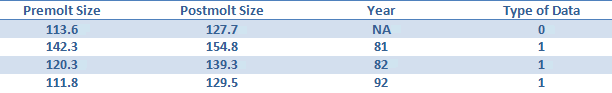
\includegraphics[width=\textwidth]{data.png}
    \end{center}
    \caption{Pattern of Data after Adjustments}
\end{figure}

\noindent In the table above, the unit of the size is millimeter and in the column of type of data, 0 represents capture-recapture data and 1 represents laboratory data.\\
Then we will focus on how premolt size changes with postmolt size for laboratory data and capture-recapture data.\\
I will use the software R to analysis the data and build the statistical model. To begin with, I will first build a linear regression model with the postmolt size and the type of data (laboratory or capture-recapture data) as the independent variables and premolt size as the dependent variable. The type of data is categorical data. 0 represents capture-recapture data and 1 represents laboratory data. Then I will find the coefficients of the two independent variables and test how significant they are to see whether the two independent variables should be included in the model. Then I will obtain an equation in the following form:
$$Premolt~Size=\beta_0 + \beta_1 (Postmolt~Size) + \beta_2 (Type~of~Data).$$ 
I will also use other methods to decide whether I should include the type of the data in the model.\\
After finishing building this simplest linear model, I will check how the model performs in predicting the dependent variable according to some criteria. If it performs well, I may stop here and regard it as the final model. But if not, I will consider about some other more complicated forms of the regression model to see how they work. For example, I may consider the form that includes the cross term:
\begin{align*}
Premolt~Size = ~&\beta_0 + \beta_1 (Postmolt~Size) + \beta_2 (Type~of~Data)\\
               & + \beta_3 (Postmolt~Size)*(Type~of~Data),
\end{align*}
or the form containing the squared term:
\begin{align*}
Premolt~Size = ~&\beta_0 + \beta_1 (Postmolt~Size) + \beta_2 (Postmolt~Size)^2\\
               & + \beta_3 (Type~of~Data).
\end{align*}
Stop when the performance of the model is satisfactory.

\section{Milestones}
We have the following major deadlines:
\begin{itemize}
    \item Work Statement due date, Sep 28, 2012,
    \item Midterm Presentation due date, Oct 12, 2012,
    \item Progress Report due date, Oct 26, 2012,
    \item Final Presentation due date, Nov 6, 2012,
    \item Final Report due date, Nov 30, 2012.
\end{itemize}

\section{Deliverable}
\subsection{From Team to Sponsor} % (fold)
The following outputs are expected from this project:
\begin{itemize}
    \item A regression formula predicting premolt sizes from postmolt sizes of female Dungeness crabs by also considering the places of molting
    \item A R programming package which can predict the premolt sizes of shells and produce a graph for the distribution of premolt sizes when people input the data of postmolt sizes of shells and the place of molting in the program
\end{itemize}

\subsection{From Sponsor to Team} % (fold)

In order for our project to be of successful one, we will need:
\begin{itemize}
    \item Data of shell sizes before molting and corresponding postmolt sizes specifying the molting environment and measurement year. The data should be delivered to me by Oct 17, 2012. If my sponsor fails to do so, I will only develop a method for the prediction problem without an explicit regression formula.
    \item Computing resources
    \item Timely responses to inquiries, 
    \item Symposium attendance travel expenses.
\end{itemize}

\newpage
\bibliographystyle{plain}
%\renewcommand\bibname{Selected Bibliography Including Cited Works}
\nocite{*}
\bibliography{Biblio}

\end{document}
